% Restructured skeleton of "Predictive Deadlock Warning", following the architecture,
% claim discipline and statistical form of the reference benchmarking paper.
% Every number below comes from the source paper's result files
% (results_ec2_c/results/c_main/eval/*.csv, c_tuning_small/*, scaling/*).
% Prose sections are scaffolds (\scaffold{...}); only the abstract is drafted in full.
% [TODO] markers are experiments or citations that do NOT exist yet. Never fill them with invented values.
\documentclass[conference]{IEEEtran}
\usepackage{iftex}
\ifXeTeX
  \usepackage{fontspec}
  \setmainfont{texgyretermes}[Extension=.otf,UprightFont=*-regular,BoldFont=*-bold,ItalicFont=*-italic,BoldItalicFont=*-bolditalic]
\else
  \usepackage[T1]{fontenc}
  \usepackage{newtxtext,newtxmath}
\fi
\usepackage{amsmath,amssymb,graphicx,booktabs,array,url,xcolor}
\usepackage[hidelinks]{hyperref}
\graphicspath{{../figures/}}

% ---- authoring macros -------------------------------------------------------
\newcommand{\scaffold}[1]{\textcolor{blue!60!black}{\textit{[Scaffold: #1]}}}
\newcommand{\todo}[1]{\textcolor{red!70!black}{\textbf{[TODO: #1]}}}
\newcommand{\todocite}{\textcolor{red!70!black}{\textbf{[TODO: cite]}}}
\newcommand{\finding}[2]{\par\smallskip\noindent\fbox{\parbox{\dimexpr\columnwidth-2\fboxsep-2\fboxrule}{\textbf{Finding #1.} #2}}\par\smallskip}
\newcommand{\anomaly}[1]{\textbf{(#1)}}

\begin{document}

\title{Predictive Deadlock Warning: Early Detection of Unsafe States from Resource-Request Patterns}

\author{\IEEEauthorblockN{Revanth Reddy Lingala}
\IEEEauthorblockA{Dept.\ of Information Technology\\
Chaitanya Bharathi Institute of Technology\\Hyderabad, India}
\and
\IEEEauthorblockN{Padigela Srujan}
\IEEEauthorblockA{Dept.\ of Information Technology\\
Chaitanya Bharathi Institute of Technology\\Hyderabad, India}}

\maketitle

% =============================================================================
\begin{abstract}
Banker's algorithm decides whether a resource-allocation state is safe now; it gives no signal that a running system is drifting towards an unsafe state, and the cost of anticipating that transition has not been measured. We measured how early, how reliably and at what compute cost a Banker-unsafe state can be anticipated, in an observer-mode simulator that grants every valid request so that unsafe states occur, over three synthetic workloads and systems of 10 to 200 processes. We compared a rule-based score over five resource-pressure indicators with a free-resource threshold, single indicators, logistic regression and gradient-boosted trees on the same signals, a scalar safety margin, a top-3 lookahead and an exact one-step lookahead, using event-level alarm precision, event recall and lead time on 150,000 test sequences (338.3 million simulation steps) disjoint from the 45,000 tuning sequences. In these configurations the rule-based score reached F1 0.28 (95\% bootstrap interval over sequences 0.28--0.28) with a median warning of 10 steps, against 0.16 for the free-resource threshold and 0.006 for random alarms at a matched rate; gradient-boosted trees on the same signals reached 0.48. On the sequences where all methods were computed, a safety margin reached 0.72 and exact lookahead 0.74, at 1.7 and 43.5 times the compute of one simulation step for 200 processes in our NumPy implementation; whether the two are equivalent is not yet tested. The state-based checks warned later (median 3--5 steps). The results describe one simulator, synthetic workloads with declared maximum claims and one implementation; intervals capture sequence-level sampling variation only, and real allocation traces and biased claim misdeclaration remain untested.
\end{abstract}

\begin{IEEEkeywords}
deadlock avoidance, Banker's algorithm, early warning, resource allocation, event-based evaluation, operating systems
\end{IEEEkeywords}

% =============================================================================
\section{Introduction}\label{sec:intro}

\scaffold{Motivation (2--3 lines): incremental resource allocation can deadlock; cite the cluster-scheduler ``temporary deadlock'' reports and resource-related outages [Jayaram2019FfDL, Lin2019DRAGON, K8sBlog2025, Gunawi2016]. Banker's algorithm is the classical avoidance test, binary and present-tense, seldom used because of its cost [Belik1987].}

\scaffold{What is known (3 groups, one sentence each): avoidance theory and complexity [Dijkstra, Habermann, Gold1978, Minoura1982]; faster safety tests [Belik1987, Finkel1987, Zohora2024]; deadlock prediction in other senses---lock-order bugs in program traces [Tunc2023, Kalhauge2018] and VM overload in a simulator [LeNgoc2023]. What is not known: the lead time, reliability and compute cost of anticipating Banker's verdict in a running allocator.}

\scaffold{Back-of-envelope expectation: unsafety is a deterministic function of (Available, Allocation, Need), so any monotone aggregate of need against free units should rise before the boundary, and a per-step safety check costs $\Theta(mn^2)$, affordable for small $n$. Why insufficient: it says nothing about how far ahead, at what false-alarm rate, which aggregate, or how cost grows with $n$ (Section~\ref{sec:related}, Table~\ref{tab:scope}).}

\scaffold{Thesis (one paragraph, scoped): in these configurations, cheap indicators anticipate unsafe states about 10 steps ahead with moderate precision (F1 0.28); non-linear combinations of the same signals reach 0.48; a fixed-budget safety check (safety margin) reaches 0.72 against 0.74 for exact lookahead at a cost that does not grow with $n$ the way exact lookahead's does, but warns later. Unexplained observations are collected in Section~\ref{sec:anomalies}.}

\scaffold{Hypotheses. State that these were formulated after an exploratory campaign and were NOT pre-registered; a pre-registered confirmatory campaign is listed in Section~\ref{sec:threats}.}
\begin{itemize}
\item \textbf{H1} (advance warning): a rule-based indicator score raises alarms before unsafe onsets with F1 above both a matched-rate random baseline and a free-resource threshold. \scaffold{Tested: Section~\ref{sec:res-accuracy}.}
\item \textbf{H2} (equivalence at lower cost): a safety check with a fixed number of Banker evaluations per step (safety margin) is equivalent in F1 to exact lookahead within $\pm\delta$, $\delta=0.05$ \todo{fix $\delta$ before the confirmatory run and justify it}, at lower cost. \scaffold{Currently two point estimates; Section~\ref{sec:res-frontier}.} \todo{paired TOST on F1 difference over independent seed batches}
\item \textbf{H3} (claim robustness): F1 of claim-based indicators is insensitive to \emph{unbiased} per-entry claim error but degrades under \emph{biased} under-claiming. \scaffold{First half measured; second half not run; Section~\ref{sec:res-robust}.} \todo{biased misdeclaration experiment}
\end{itemize}

\scaffold{Contributions.}
\begin{enumerate}
\item[C1] \scaffold{The measured advance-warning result: per-method alarm precision, event recall and lead time for 12 methods on 150,000 test sequences, with the workload regimes in which warning quality holds or fails (Sections~\ref{sec:res-accuracy}--\ref{sec:res-workload}).}
\item[C2] \scaffold{The cost--accuracy--lead-time frontier, with compute measured per method and stated as an instrument effect of our implementation (Section~\ref{sec:res-frontier}).}
\item[C3] \scaffold{An evaluation protocol for deadlock early warning adapted from clinical and seismic early warning, with an observer-mode simulator and 134 tests (Section~\ref{sec:method}).}
\end{enumerate}
\scaffold{Secondary results: unsafe-vs-deadlock outcomes as a model property (Section~\ref{sec:res-deadlock}); horizon sensitivity; scaling of the vectorised safety check. The simulator and pipeline are an artifact, not a contribution.}

\scaffold{Scope paragraph: one simulator, three synthetic workloads, declared maximum claims, fixed process sets, one NumPy implementation, one AWS instance type; no real allocation traces, no avoidance acting on warnings, no distributed setting.}

% =============================================================================
\section{Background and Related Work}\label{sec:related}

\subsection{Banker's Algorithm, Unsafe States and Deadlock}\label{sec:bg-banker}
\scaffold{Define Max, Allocation, Need, Available; the safety test and its $\Theta(mn^2)$ cost [Dijkstra-EWD623, Habermann1969, Belik1987]. Safe/unsafe/deadlocked: never safe and deadlocked; unsafe need not deadlock [Holt1972, Silberschatz2018]; safety is not liveness [Holt1971, ParnasHabermann1972]. Dijkstra's definition is the ground truth of every metric in this paper.}

\subsection{Related Measurements}\label{sec:bg-related}
\scaffold{Table~\ref{tab:scope} positions this study. Say explicitly: entries describe the scope of each work, not shortcomings. One paragraph per group, compressed from the source's seven-theme survey: (i) avoidance theory and complexity of ``deadlock prediction'' as a static decision [Gold1978, Minoura1982, Kameda1980]; (ii) faster safety tests [Belik1987, Finkel1987, LiCook2007, Zohora2024], two of which inspire our margin and lookahead baselines [Finkel1987, AndrewsLevin1982]; (iii) detection after formation [Agrawal1983, Chandy1983, Knapp1987, Singhal1989]; (iv) program lock-deadlock prediction [Bensalem2006, Joshi2009, Kalhauge2018, Tunc2023]; (v) learning-based resource prediction [LeNgoc2023, Oluwaseyi2024 (preprint)]; (vi) deadlock control outside operating systems [Banaszak1990, Ezpeleta1995, Fanti2004, Li2008].}

\begin{table*}[t]
\centering\footnotesize
\caption{Scope of related work. \checkmark\ = covered; -- = outside the study's scope or not reported. P = peer-reviewed, A = preprint. Entries describe scope, not shortcomings.}
\label{tab:scope}
\begin{tabular}{>{\raggedright\arraybackslash}p{3.3cm}c>{\raggedright\arraybackslash}p{4.2cm}ccccc}
\toprule
Study & Type & Setting & Banker safety & Forecast of transition & Lead time & Event-based eval. & Cost per method \\
\midrule
Dijkstra; Habermann & P & Avoidance by safety test & \checkmark & -- & -- & -- & -- \\
Gold; Minoura; Kameda & P & Complexity of deciding avoidability & \checkmark & -- & -- & -- & complexity \\
Belik; Finkel \& Madduri; DBDAA & P & Faster or dynamic safety tests & \checkmark & -- & -- & -- & \checkmark \\
Andrews \& Levin & P & Safety of prospective requests & \checkmark & -- & -- & -- & -- \\
Agrawal et al.; Chandy et al. & P & Deadlock detection (databases, distributed) & -- & -- & -- & -- & \checkmark \\
Kalhauge \& Palsberg; Tun\c{c} et al. & P & Lock-order deadlocks in program traces & -- & -- & -- & -- & \checkmark \\
Le Ngoc \& Tran Cong & P & ML load balancing in CloudSim & -- & \checkmark & -- & -- & -- \\
Oluwaseyi & A & AI thread-deadlock prediction (proposal) & -- & \checkmark & -- & -- & -- \\
Ezpeleta et al.; Li et al. & P & Petri-net deadlock control (manufacturing) & -- & -- & -- & -- & -- \\
Hyland et al.; M\"unchmeyer et al. & P & Clinical / seismic early warning & -- & \checkmark & \checkmark & \checkmark & -- \\
\textbf{This work} & & Early warning of Banker-unsafe states & \checkmark & \checkmark & \checkmark & \checkmark & \checkmark \\
\bottomrule
\end{tabular}
\end{table*}

\scaffold{Dated search statement (honest, as in the reference): ``In October 2026 we ran keyword searches \todo{list exact databases actually searched, e.g.\ Crossref/OpenAlex/Semantic Scholar via the research tool, and the date} combining \emph{Banker's algorithm}, \emph{deadlock prediction}, \emph{deadlock avoidance}, \emph{unsafe state} and \emph{early warning}; the queries and results are logged in the artifact \todo{save the query log into the repository}. This is a keyword search, not a systematic review; it did not cover IEEE Xplore or Google Scholar directly, which limits the statement that no prior work measures this.''}

\subsection{Early-Warning Evaluation Method}\label{sec:bg-method}
\scaffold{Three strands inform the design: (1) event-level recall/precision and alarm silencing from clinical early warning [Hyland2020]---our problem has the same structure (rare harmful state change, continuous monitoring, value only if early); (2) warning time traded against precision along thresholds, alarm at onset counted as a miss [Munchmeyer2021]; (3) range-based and window-based scoring [Tatbul2018, Lavin2015], PR over ROC for rare events [Saito2015, Davis2006], bootstrap intervals [Efron1993]. For equivalence we will follow two one-sided tests \todocite.}

% =============================================================================
\section{Design and Threat Model}\label{sec:design}

\scaffold{Observer mode: every valid request is granted; Banker's check and detection only observe; this is what lets unsafe states occur. Step loop in five stages. Ground truth: unsafe onset (primary), deadlock onset (secondary); flicker merging with a 5-step gap; onsets in the first 3 steps excluded.}

\scaffold{Workloads: normal (small requests, early releases), spike (80\% of processes grab 30--60\% of remaining need once 20--60\% of initial need is requested), deadlock-prone (process $i$ prefers resource $(i{+}1)\bmod m$). Claim tightness calibrated on tuning seeds (1.43, 1.58, 1.48 realised; Table~\ref{tab:setup}).}

\scaffold{Out of scope (explicit list): real allocation traces; process arrivals; avoidance that acts on a warning; distributed or multi-node allocators; preemption and recovery; workloads whose processes stop short of their claims; adversarial request streams.}

\begin{table}[t]
\centering\footnotesize
\caption{Methods compared. All use the same alarm rule (threshold, $k$, refractory $R$) tuned on the tuning split. Cost is extra compute per step relative to one simulation step at 200 processes (Table~\ref{tab:cost}).}
\label{tab:methods}
\begin{tabular}{>{\raggedright\arraybackslash}p{2.1cm}>{\raggedright\arraybackslash}p{2.9cm}cc}
\toprule
Method & Signal & Trained & Cost \\
\midrule
Random & Bernoulli, matched rate & no & $\approx$0 \\
Availability & free fraction of units & no & $\approx$0 \\
Single indicators (4) & one of need pressure, contention, waiting ratio, request rate & no & $\approx$0 \\
Combined (ours) & weighted mean of 5 indicators & no & $\approx$0 \\
Combined, max & weighted maximum & no & $\approx$0 \\
Logistic regression & 5 indicators + 10-step changes & yes & $\approx$0 \\
Boosted trees & same features & yes & $\approx$0 \\
Safety margin & binary search over free units (7 checks) & no & 1.66 \\
Top-3 lookahead & $\le$3 prospective-grant checks & no & 0.91 \\
Exact lookahead & 1 check per running process & no & 43.45 \\
\bottomrule
\end{tabular}
\end{table}

\begin{table}[t]
\centering\footnotesize
\caption{Claim taxonomy}
\label{tab:claims}
\begin{tabular}{>{\raggedright\arraybackslash}p{1.6cm}>{\raggedright\arraybackslash}p{2.9cm}>{\raggedright\arraybackslash}p{2.9cm}}
\toprule
Class & Claimed & Not claimed \\
\midrule
Correctness & Simulator invariants, vectorised = reference safety and detection on 2,000 random states, deadlocked $\Rightarrow$ unsafe (134 tests) & Formal proof of the simulator \\
Warning accuracy & Measured precision, recall, F1, lead time in these workloads and sizes & Accuracy on real systems or other workload families \\
Equivalence & -- & That safety margin and exact lookahead are equivalent (\todo{TOST}) \\
Cost & Measured per-step compute of our NumPy implementation & Cost of other implementations or of incremental safety tests \\
Deadlock outcome & Fraction of unsafe episodes ending in deadlock under this simulator & That unsafe states usually deadlock in real systems \\
Robustness & Insensitivity to unbiased $\pm$20\% per-entry claim error & Robustness to biased or systematic misdeclaration \\
Out of scope & -- & Avoidance acting on warnings, distributed allocators, process arrivals \\
\bottomrule
\end{tabular}
\end{table}

% =============================================================================
\section{Implementation and Methodology}\label{sec:method}

\subsection{Implementation}\label{sec:impl}
\scaffold{Python simulator with NumPy-vectorised safety check (verified against the textbook loop), event-driven deadlock detection (verified against every-step detection), per-step indicators and state-based baselines recorded on a separate random stream. Pinned versions: Python 3.12.3 (EC2), NumPy 2.4.6, pandas 3.0.6, PyArrow 25.0.1, scikit-learn 1.9.1. 134 automated tests covering every row of the edge-case matrix. Analysis pipeline generates every number and table as \LaTeX\ macros.}

\subsection{Testbed and Workloads}\label{sec:testbed}
\scaffold{Three campaigns, never pooled (Table~\ref{tab:campaigns}). The tuning and test seed ranges are disjoint (asserted in code). Testbed: one AWS EC2 c7i.8xlarge (32 vCPU, 61 GB), region ap-south-2, Ubuntu 24.04; 32 worker processes, one OpenMP/BLAS thread each. Cost guards and audit. Commit hashes recorded per run.}

\begin{table}[t]
\centering\footnotesize
\caption{Campaigns. Results are never pooled across campaigns; this paper reports the full-paper campaign unless stated.}
\label{tab:campaigns}
\begin{tabular}{>{\raggedright\arraybackslash}p{1.7cm}rrr>{\raggedright\arraybackslash}p{1.6cm}}
\toprule
Campaign & Sequences & Steps & Cost & Role \\
\midrule
Mac dry run & 48,000 & 55.7\,M & -- & pipeline check (exploratory) \\
EC2 Option B & 300,000 & 676.2\,M & \$4.11 & first cloud campaign (exploratory) \\
EC2 full paper & 195,000 & 439.6\,M & \$8.39 & results of record \\
\bottomrule
\end{tabular}
\end{table}

\begin{table*}[t]
\centering
\footnotesize
\caption{Experimental setup per cell (test split). Test split: 150,000 sequences, 338,262,425 steps; tuning split: 45,000 sequences, 101,341,468 steps. Machine: Linux-7.0.0-1014-aws-x86\_64-with-glibc2.39 (32 CPUs, c7i.8xlarge).}
\label{tab:setup}
\begin{tabular}{lrrrrrrrr}
\toprule
scenario & n & m & seqs & steps & events & \% with event & \% deadlock & tightness \\
\midrule
normal & 10 & 5 & 10{,}000 & 1{,}071{,}547 & 2{,}754 & 26.90 & 25.40 & 1.43 \\
normal & 25 & 8 & 10{,}000 & 4{,}494{,}155 & 1{,}674 & 15.70 & 14.30 & 1.43 \\
normal & 50 & 10 & 10{,}000 & 11{,}527{,}074 & 1{,}270 & 11.30 & 10.10 & 1.43 \\
normal & 100 & 20 & 10{,}000 & 39{,}280{,}274 & 8{,}469 & 65.80 & 62.70 & 1.43 \\
normal & 200 & 20 & 10{,}000 & 82{,}123{,}372 & 7{,}358 & 56.20 & 53.60 & 1.43 \\
spike & 10 & 5 & 10{,}000 & 707{,}662 & 7{,}066 & 70.70 & 70.70 & 1.58 \\
spike & 25 & 8 & 10{,}000 & 2{,}939{,}715 & 5{,}954 & 59.50 & 59.50 & 1.58 \\
spike & 50 & 10 & 10{,}000 & 7{,}434{,}425 & 5{,}317 & 53.20 & 53.20 & 1.58 \\
spike & 100 & 20 & 10{,}000 & 27{,}023{,}589 & 6{,}185 & 61.90 & 61.90 & 1.58 \\
spike & 200 & 20 & 10{,}000 & 56{,}973{,}051 & 5{,}346 & 53.50 & 53.50 & 1.58 \\
deadlock\_prone & 10 & 5 & 10{,}000 & 1{,}020{,}230 & 4{,}073 & 40.70 & 40.70 & 1.48 \\
deadlock\_prone & 25 & 8 & 10{,}000 & 4{,}036{,}769 & 4{,}047 & 40.50 & 40.50 & 1.48 \\
deadlock\_prone & 50 & 10 & 10{,}000 & 9{,}877{,}410 & 4{,}513 & 45.10 & 45.10 & 1.48 \\
deadlock\_prone & 100 & 20 & 10{,}000 & 29{,}793{,}804 & 9{,}316 & 93.20 & 93.20 & 1.48 \\
deadlock\_prone & 200 & 20 & 10{,}000 & 59{,}959{,}348 & 9{,}270 & 92.70 & 92.70 & 1.48 \\
\bottomrule
\end{tabular}
\end{table*}

% Table II of the source: per-cell setup of the test split (150,000 sequences, 338,262,425 steps).

\subsection{Statistical Analysis}\label{sec:stats}
\scaffold{Metrics: event-level precision and recall [Hyland2020], F1, false alarms and alarms per 1,000 steps, lead time, NAB-style score [Lavin2015]. Tuning: threshold 5--95, $k\in\{1,2,3\}$, $R\in\{10,20\}$, weights for combinations; maximise F1 subject to $\le$5 false alarms per 1,000 steps and median lead $\ge$3, on tuning seeds; learned models trained on even and thresholded on odd tuning seeds.}

\scaffold{Experimental unit (the key change): the current intervals (e.g.\ F1 0.28 [0.28, 0.28]) resample sequences from one generator and so capture only sequence-level sampling variance; they are not intervals over independent replications. Proposed unit: an independent batch of seeds (or a claim-tightness setting), with methods compared by paired differences within each batch.} \todo{re-run the test split as $B\ge20$ independent seed batches per cell (e.g.\ 20 batches of 500 seeds) and report paired F1 differences with batch-level intervals}

\scaffold{Equivalence: H2 is tested with two one-sided tests on the paired batch-level F1 difference against $\pm\delta$; non-equivalent if the interval lies outside, otherwise inconclusive---never ``no difference''.} \todo{paired TOST on F1 difference (safety margin vs exact lookahead), on the common subset}

\scaffold{Deviations and post-hoc choices (list honestly): (1) tuning split reduced from 10,000 to 3,000 seeds per cell after a pilot projected the run past its time gate; (2) tuning, evaluation and figures re-run after two bugs found mid-run (thread oversubscription; NaN in the learned-score prior correction), simulation data unaffected; (3) the spike workload was redesigned after calibration showed it produced no unsafe states; (4) the paired lead-time comparison, NAB score and per-size table were chosen after seeing data; (5) hypotheses H1--H3 were written after the exploratory campaigns. None of the analyses was pre-registered.} \todo{pre-register hypotheses, margin $\delta$, primary cells and batch count before a confirmatory campaign}

% =============================================================================
\section{Results}\label{sec:results}

\subsection{Per-Method Accuracy and Lead Time}\label{sec:res-accuracy}
\scaffold{Table~\ref{tab:main} on the full test population. Note the population difference: exact lookahead was computed on a seed subset; its row is therefore reported only on the common subset (Table~\ref{tab:common}), where all methods are compared on identical sequences. Report effects with intervals; separate the common-subset comparison (pre-specified) from the full-population table.}

\begin{table*}[t]
\centering\footnotesize
\caption{Per-method results on the full test population (unsafe target, $H_{\max}=20$, 150,000 sequences, 82,612 onsets). Intervals: 95\% bootstrap over sequences, stratified by workload and size (sequence-level sampling variance only). Exact lookahead is omitted here because it was computed on a subset; see Table~\ref{tab:common}.}
\label{tab:main}
\begin{tabular}{lcccccc}
\toprule
Method & Precision & Recall & F1 [95\% CI] & FA/1000 & Median lead & NAB \\
\midrule
Combined (ours) & 0.236 & 0.344 & 0.280 [0.277, 0.283] & 0.333 & 10 & 22.1 \\
Contention & 0.300 & 0.388 & 0.338 [0.336, 0.341] & 0.221 & 7 & 27.2 \\
Combined, max & 0.300 & 0.388 & 0.338 [0.336, 0.341] & 0.221 & 7 & 27.2 \\
Need pressure & 0.314 & 0.136 & 0.190 [0.187, 0.193] & 0.072 & 7 & 9.5 \\
Waiting ratio & 0.242 & 0.259 & 0.250 [0.248, 0.252] & 0.307 & 13 & 16.6 \\
Request rate & 0.161 & 0.116 & 0.135 [0.133, 0.137] & 0.148 & 9 & 6.6 \\
Availability & 0.106 & 0.344 & 0.162 [0.160, 0.164] & 0.708 & 8 & 13.0 \\
Logistic regression & 0.240 & 0.435 & 0.310 [0.307, 0.312] & 0.480 & 12 & 28.3 \\
Boosted trees & 0.406 & 0.579 & 0.477 [0.475, 0.480] & 0.292 & 11 & 45.0 \\
Safety margin & 0.639 & 0.611 & 0.625 [0.622, 0.627] & 0.084 & 4 & 43.8 \\
Top-3 lookahead & 0.541 & 0.617 & 0.576 [0.574, 0.579] & 0.128 & 5 & 45.6 \\
Random (matched rate) & 0.005 & 0.009 & 0.006 [0.006, 0.006] & 0.438 & 11 & -- \\
\bottomrule
\end{tabular}
\end{table*}

\begin{table}[t]
\centering\footnotesize
\caption{All methods on the common subset where exact lookahead was computed (61,350 sequences: all with $n\le25$, 200 seeds per cell for $n=50,100$, 50 for $n=200$; 26,382 onsets). Same intervals as Table~\ref{tab:main}.}
\label{tab:common}
\begin{tabular}{lccc}
\toprule
Method & F1 [95\% CI] & FA/1000 & Lead \\
\midrule
Exact lookahead & 0.745 [0.741, 0.749] & 0.624 & 4 \\
Safety margin & 0.718 [0.714, 0.722] & 0.543 & 4 \\
Top-3 lookahead & 0.693 [0.689, 0.698] & 0.683 & 5 \\
Boosted trees & 0.539 [0.535, 0.543] & 2.394 & 10 \\
Contention & 0.515 [0.510, 0.520] & 1.039 & 6 \\
Combined (ours) & 0.443 [0.437, 0.448] & 0.481 & 5 \\
Logistic regression & 0.362 [0.359, 0.365] & 5.442 & 12 \\
Request rate & 0.333 [0.327, 0.338] & 0.516 & 8 \\
Availability & 0.298 [0.292, 0.303] & 0.351 & 4 \\
Need pressure & 0.182 [0.176, 0.187] & 0.084 & 4 \\
Waiting ratio & 0.141 [0.136, 0.146] & 0.320 & 4 \\
Random & 0.014 [0.013, 0.014] & 0.422 & 9 \\
\bottomrule
\end{tabular}
\end{table}

\scaffold{Ablation (Table~\ref{tab:ablation}): removing contention lowers the equal-weight mean from 0.239 to 0.198, removing waiting ratio raises it to 0.267; averaging dilutes the strongest indicator. The tuned weights double contention, under which the weighted maximum coincides with contention alone.}
\begin{table}[t]
\centering
\footnotesize
\caption{Ablation: combined score with one indicator removed (each re-tuned on the tuning split).}
\label{tab:ablation}
\begin{tabular}{lrrrr}
\toprule
variant & precision & recall & F1 & FA/1000 \\
\midrule
all five, equal & 0.17 & 0.40 & 0.24 & 0.59 \\
without scarcity & 0.19 & 0.39 & 0.26 & 0.47 \\
without need\_pressure & 0.17 & 0.45 & 0.25 & 0.64 \\
without contention & 0.14 & 0.36 & 0.20 & 0.65 \\
without waiting\_ratio & 0.23 & 0.31 & 0.27 & 0.30 \\
without request\_rate & 0.15 & 0.41 & 0.22 & 0.93 \\
\bottomrule
\end{tabular}
\end{table}


\begin{figure}[t]\centering
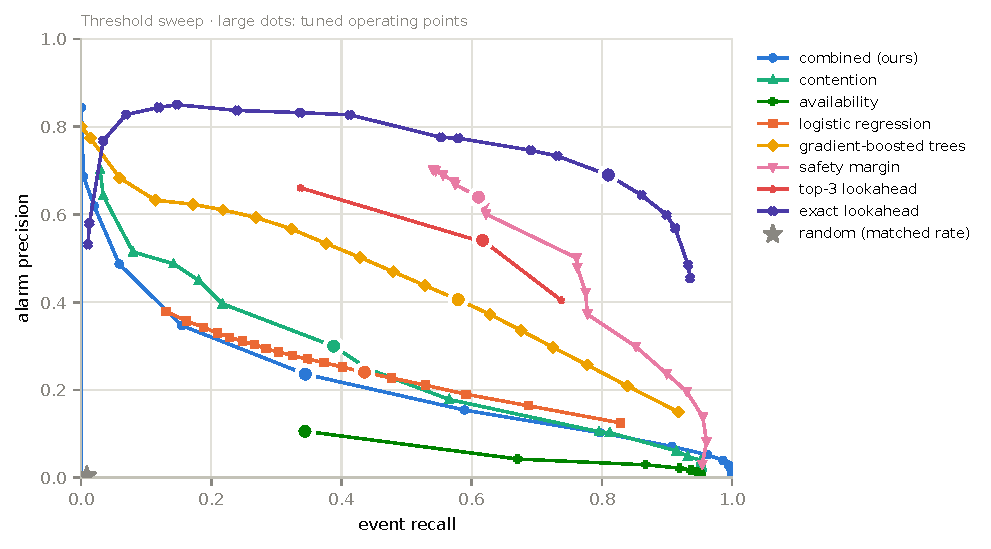
\includegraphics[width=\columnwidth]{fig3_pr_curves.pdf}
\caption{Precision--recall along each threshold sweep (test split, not used for selection).}\label{fig:pr}
\end{figure}

\finding{1}{In these configurations the rule-based score warned a median 10 steps ahead with F1 0.28, above the free-resource threshold (0.16) and matched-rate random alarms (0.006); boosted trees on the same signals reached 0.48. Intervals are over sequences, not independent replications.}

\subsection{Where Warning Quality Varies}\label{sec:res-workload}
\scaffold{Table~\ref{tab:scenario}: spike easiest for most methods; gradual build-ups hardest for aggregate indicators; state-based checks degrade least. Per-size: F1 declines at larger $n$ (anomaly A4 (Section~\ref{sec:anomalies})). Waiting ratio's reversal on spike is anomaly A1.}
\begin{table}[t]
\centering
\footnotesize
\caption{F1 per scenario (unsafe target, $H_{max}=20$).}
\label{tab:scenario}
\begin{tabular}{lrrr}
\toprule
method & deadlock\_prone & spike & normal \\
\midrule
combined & 0.23 & 0.42 & 0.22 \\
need\_pressure & 0.01 & 0.34 & 0.06 \\
contention & 0.22 & 0.49 & 0.21 \\
waiting\_ratio & 0.31 & 0.03 & 0.29 \\
request\_rate & 0.00 & 0.23 & 0.00 \\
availability & 0.05 & 0.34 & 0.10 \\
lookahead & 0.69 & 0.83 & 0.66 \\
random & 0.01 & 0.01 & 0.00 \\
\bottomrule
\end{tabular}
\end{table}


\finding{2}{Warning quality depended on how danger built up: the rule-based score reached F1 0.42 on spike workloads and 0.22--0.23 on gradual ones; unsafe onsets followed a median 26 steps after a spike began (3.0\% before it).}

\subsection{Cost--Accuracy Frontier}\label{sec:res-frontier}
\scaffold{Table~\ref{tab:cost} and Fig.~\ref{fig:frontier}. State the instrument effect: costs are those of our NumPy-vectorised safety check (one check 59.9\,$\mu$s on average; textbook loop 1.3--7.7$\times$ slower, Table~\ref{tab:scaling}); a different implementation or an incremental safety test [Belik1987, Finkel1987] would move every state-based point, so ratios, not absolute times, are the result. H2 is currently two point estimates (0.718 vs 0.745 on the common subset); report it as \emph{inconclusive} until the paired TOST is run.}
\begin{table}[t]
\centering
\footnotesize
\caption{Measured compute per step (test split). A simulation step includes one safety check and the indicators; learned models add a few vector operations.}
\label{tab:cost}
\begin{tabular}{lrrr}
\toprule
computation & processes & $\mu$s/step & $\times$ simulation step \\
\midrule
simulation step & all & 289.18 & 1.00 \\
one safety check & all & 59.89 & 0.21 \\
safety margin & all & 417.28 & 1.44 \\
safety margin & 200 & 479.30 & 1.66 \\
top-3 lookahead & all & 231.46 & 0.80 \\
top-3 lookahead & 200 & 264.00 & 0.91 \\
exact lookahead & all & 1850.09 & 6.40 \\
exact lookahead & 200 & 12565.63 & 43.45 \\
\bottomrule
\end{tabular}
\end{table}

\begin{figure}[t]\centering
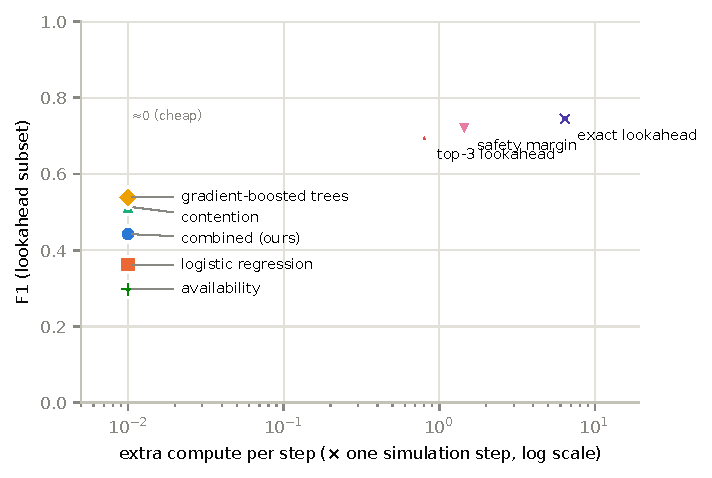
\includegraphics[width=\columnwidth]{fig9_cost_frontier.pdf}
\caption{F1 on the common subset against extra compute per step (log scale).}\label{fig:frontier}
\end{figure}
\begin{figure}[t]\centering
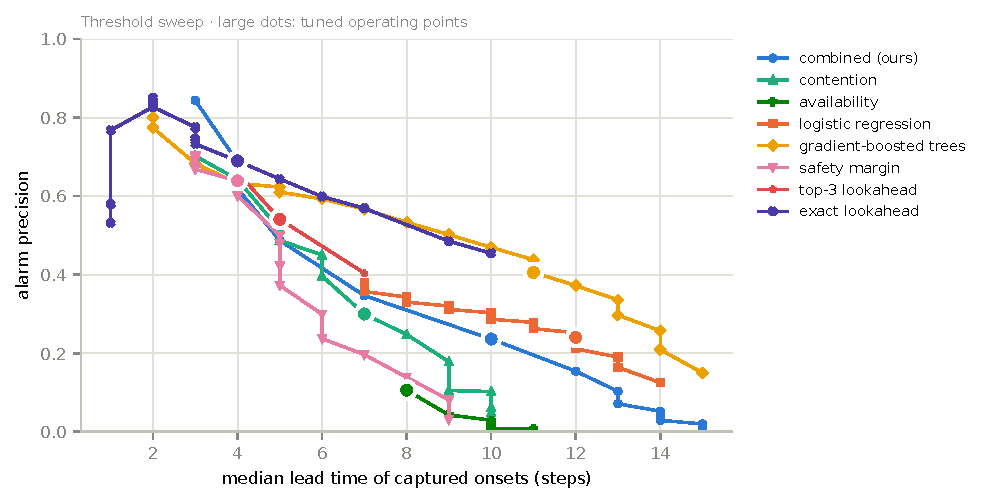
\includegraphics[width=\columnwidth]{fig10_precision_lead.pdf}
\caption{Precision against median lead time along each threshold sweep.}\label{fig:leadprec}
\end{figure}

\finding{3}{On the common subset the safety margin reached F1 0.72 and exact lookahead 0.74, at 1.7$\times$ and 43.5$\times$ one simulation step for 200 processes in our implementation; equivalence is not yet tested \todo{paired TOST}. State-based checks warned later (median 3--5 steps) than the cheap signals (7--13).}

\subsection{Unsafe States and Deadlock}\label{sec:res-deadlock}
\scaffold{Present as a property of the model, not of systems: 100\% of resolved unsafe episodes ended in deadlock under spike (29,868) and deadlock-prone (31,219), 77.2\% under normal (16,613 of 21,525), because processes eventually request full claims and sequences end at the first deadlock; caveat in Section~\ref{sec:threats}. Deadlock target (Table~\ref{tab:deadlock}): label the exact-lookahead row's different population (25,862 vs 77,700 onsets).}
\begin{table}[t]
\centering\footnotesize
\caption{Deadlock-onset target, $H_{\max}=20$ (alarms not masked while unsafe). The exact-lookahead row is computed on a different population (25,862 onsets) and is not comparable with the others (77,700).}
\label{tab:deadlock}
\begin{tabular}{lcccr}
\toprule
Method & Precision & Recall & F1 & Onsets \\
\midrule
Waiting ratio & 0.333 & 0.833 & 0.476 & 77,700 \\
Boosted trees & 0.314 & 0.985 & 0.476 & 77,700 \\
Combined (ours) & 0.212 & 0.708 & 0.326 & 77,700 \\
Logistic regression & 0.183 & 0.654 & 0.286 & 77,700 \\
Contention & 0.173 & 0.543 & 0.262 & 77,700 \\
Need pressure & 0.178 & 0.344 & 0.235 & 77,700 \\
Availability & 0.095 & 0.521 & 0.161 & 77,700 \\
Safety margin & 0.144 & 0.169 & 0.155 & 77,700 \\
Top-3 lookahead & 0.111 & 0.151 & 0.128 & 77,700 \\
Request rate & 0.072 & 0.058 & 0.064 & 77,700 \\
Random & 0.005 & 0.009 & 0.006 & 77,700 \\
\midrule
Exact lookahead$^\dagger$ & 0.320 & 0.434 & 0.369 & 25,862 \\
\bottomrule
\end{tabular}
\\[2pt]{\scriptsize $^\dagger$ different population; \todo{recompute all rows on the common subset}}
\end{table}
\begin{table*}[t]
\centering
\footnotesize
\caption{Unsafe-episode outcomes per scenario.}
\label{tab:episodes}
\begin{tabular}{lrrrrr}
\toprule
scenario & ep\_recovered & ep\_deadlocked & ep\_censored & recovered\_frac & deadlocked\_frac \\
\midrule
deadlock\_prone & 0 & 31{,}219 & 0 & 0.00 & 1.00 \\
normal & 4{,}912 & 16{,}613 & 0 & 0.23 & 0.77 \\
spike & 0 & 29{,}868 & 0 & 0.00 & 1.00 \\
\bottomrule
\end{tabular}
\end{table*}


\finding{4}{Under this simulator, unsafe episodes ended in deadlock in 77--100\% of cases; this follows partly from design (full-claim requests, sequences end at the first deadlock) and is not a claim about real systems.}

\subsection{Robustness to Misdeclared Claims}\label{sec:res-robust}
\scaffold{Table~\ref{tab:robust}: with independent per-entry multiplicative error $U(0.8,1.2)$, F1 changed by at most 0.004. Limitation: per-entry errors are zero-mean and cancel in the aggregates (sums over processes and resources), so this does not test systematic misdeclaration. H3's second half is untested.}
\begin{table}[t]
\centering
\footnotesize
\caption{Robustness: the same tuned rules when need pressure and contention are computed from maximum claims misdeclared by up to $\pm$20\% (ground truth uses the true claims).}
\label{tab:robust}
\begin{tabular}{lrrr}
\toprule
method & F1, true claims & F1, claims $\pm$20\% & change \\
\midrule
combined (ours) & 0.280 & 0.280 & +0.000 \\
combined, max & 0.338 & 0.337 & -0.001 \\
need pressure & 0.190 & 0.194 & +0.004 \\
contention & 0.338 & 0.337 & -0.001 \\
logistic regr. & 0.310 & 0.311 & +0.002 \\
boosted trees & 0.477 & 0.476 & -0.001 \\
\bottomrule
\end{tabular}
\end{table}

\todo{biased misdeclaration experiment: all claims scaled by a common factor (e.g.\ 0.8 and 0.9, systematic under-claiming; 1.1 and 1.2, over-claiming) for indicators, ground truth on true claims}

\finding{5}{Unbiased per-entry claim error of up to $\pm$20\% changed F1 by at most 0.004 for every claim-based method; biased misdeclaration was not tested.}

\subsection{Horizon Sensitivity}\label{sec:res-horizon}
\scaffold{Table~\ref{tab:hmax}: same alarms, wider horizon raises F1 for every method (combined 0.108, 0.190, 0.280, 0.399 for $H_{\max}$ 5--50); many alarms precede onsets by more than 20 steps. Analysis chosen before the full-paper run (exploratory in Option B).}
\begin{table}[t]
\centering\footnotesize
\caption{F1 against warning horizon $H_{\max}$ (same alarms).}
\label{tab:hmax}
\begin{tabular}{lcccc}
\toprule
Method & 5 & 10 & 20 & 50 \\
\midrule
Combined (ours) & 0.108 & 0.190 & 0.280 & 0.399 \\
Contention & 0.129 & 0.222 & 0.338 & 0.432 \\
Boosted trees & 0.178 & 0.330 & 0.477 & 0.597 \\
Safety margin & 0.374 & 0.490 & 0.625 & 0.707 \\
Top-3 lookahead & 0.295 & 0.433 & 0.576 & 0.691 \\
Exact lookahead$^\dagger$ & 0.482 & 0.648 & 0.745 & 0.798 \\
Availability & 0.055 & 0.097 & 0.162 & 0.251 \\
Random & 0.002 & 0.003 & 0.006 & 0.015 \\
\bottomrule
\end{tabular}
\\[2pt]{\scriptsize $^\dagger$ common subset only.}
\end{table}

\finding{6}{Widening the horizon from 5 to 50 steps raised every method's F1 (rule-based 0.11 to 0.40); the ranking of methods did not change.}

\subsection{Scaling of the Safety Check}\label{sec:res-scaling}
\scaffold{Table~\ref{tab:scaling}, Fig.~\ref{fig:scaling}: vectorised 1.3--7.7$\times$ faster than the textbook loop; log--log slope in $n$ 0.29 (vectorised) and 0.77 (reference) at $m=20$, far below the $\Theta(mn^2)$ worst case---an average-case observation for these workloads and this implementation, consistent with [Belik1987].}
\begin{table}[!htb]
\centering
\footnotesize
\caption{Runtime scaling: time per Banker's safety check on random valid states (vectorised vs. reference) and whole-simulator time per step.}
\label{tab:scaling}
\begin{tabular}{lrrrrr}
\toprule
n & m & vec $\mu$s & ref $\mu$s & speed-up & $\mu$s/step \\
\midrule
10 & 5 & 7.1 & 9.7 & 1.4 & 100.7 \\
10 & 10 & 6.9 & 9.4 & 1.4 & 103.0 \\
10 & 20 & 6.9 & 10.5 & 1.5 & 103.7 \\
25 & 5 & 9.0 & 19.5 & 2.2 & 101.2 \\
25 & 10 & 7.4 & 17.6 & 2.4 & 104.6 \\
25 & 20 & 7.4 & 17.3 & 2.3 & 107.5 \\
50 & 5 & 9.1 & 29.6 & 3.3 & 102.1 \\
50 & 10 & 8.1 & 28.4 & 3.5 & 113.3 \\
50 & 20 & 9.0 & 28.6 & 3.2 & 118.8 \\
100 & 5 & 12.1 & 60.8 & 5.0 & 110.0 \\
100 & 10 & 9.9 & 51.9 & 5.3 & 118.0 \\
100 & 20 & 11.2 & 54.3 & 4.9 & 118.9 \\
200 & 5 & 17.8 & 138.0 & 7.7 & 129.1 \\
200 & 10 & 13.7 & 103.3 & 7.6 & 131.7 \\
200 & 20 & 15.6 & 99.7 & 6.4 & 141.6 \\
\bottomrule
\end{tabular}
\end{table}

\begin{figure}[t]\centering
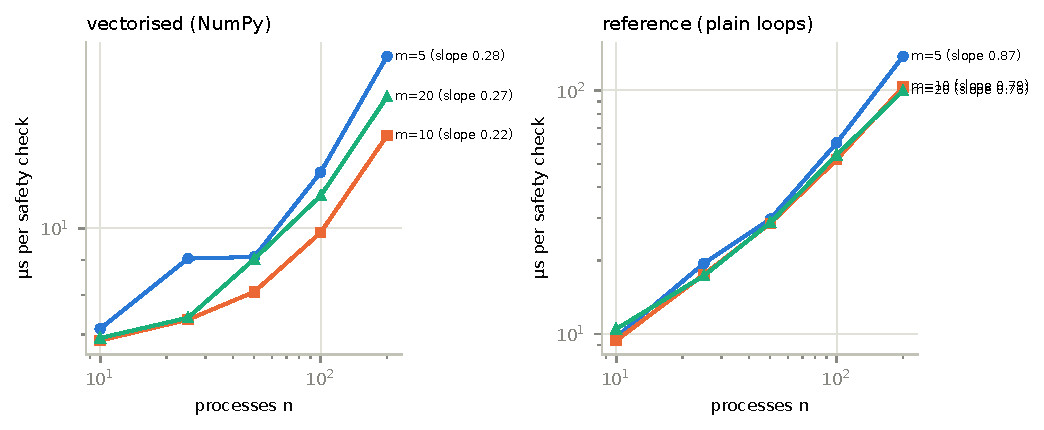
\includegraphics[width=\columnwidth]{fig7_scaling.pdf}
\caption{Time per safety check against $n$ (log--log).}\label{fig:scaling}
\end{figure}

\finding{7}{The vectorised safety check grew far more slowly than $\Theta(mn^2)$ in these workloads (slope 0.29 at $m=20$); this is average-case behaviour of one implementation.}

\subsection{Open Anomalies}\label{sec:anomalies}
\scaffold{Six observations are not explained by anything above. Each: what was observed (numbers), what was checked, candidate explanation, and the experiment that would resolve it.}
\begin{enumerate}
\item[\anomaly{A1}] \scaffold{Waiting ratio scores F1 0.288 (normal) and 0.305 (deadlock-prone) but 0.030 on spike (recall 0.016, 1,402 alarms for 29,868 onsets). Candidate: spikes are granted grabs capped by free units, so few processes block before the onset. Not tested.} \todo{per-workload waiting-count trace before onsets}
\item[\anomaly{A2}] \scaffold{Boosted trees reach recall 0.985 on the deadlock target at $H_{\max}=20$ (0.992 at 50) with precision 0.314---near-saturated recall that no other method approaches. Candidate: unmasked alarms during long unsafe episodes preceding deadlock. Not tested.} \todo{deadlock-target recall restricted to alarms raised while safe}
\item[\anomaly{A3}] \scaffold{Safety margin (0.155) and top-3 lookahead (0.128) score at or below availability (0.161) on the deadlock target despite leading on the unsafe target. Candidate: both are computed only on safe steps, so they are silent during the unsafe episodes that precede deadlock---a construction effect.} \todo{compute both during unsafe steps and re-evaluate}
\item[\anomaly{A4}] \scaffold{F1 falls with system size beyond $n=25$ for every method: rule-based 0.470 ($n=25$) to 0.197 ($n=200$), exact lookahead 0.756 ($n=10$) to 0.534, safety margin 0.722 to 0.509; the decline is not monotone for the rule-based score (0.433 at $n=10$). Candidate: thresholds are tuned once across sizes; onset density differs by size. Not tested.} \todo{per-size tuning}
\item[\anomaly{A5}] \scaffold{Request rate F1 is 0.001 (normal) and 0.000 (deadlock-prone) against 0.230 (spike); need pressure is 0.010 on deadlock-prone; three single-indicator baselines chose the top of the threshold grid (95).} \todo{extend threshold grid above 95}
\item[\anomaly{A6}] \scaffold{Logistic regression raises 5.44 false alarms per 1,000 steps on the common subset against 0.480 overall; thresholds tuned on all sizes may not transfer to the small-$n$ subset.}
\end{enumerate}

% =============================================================================
\section{Threats to Validity}\label{sec:threats}
\scaffold{Internal: intervals capture sequence sampling of one generator, not run-to-run variation (Section~\ref{sec:stats}); hypotheses and several analyses were chosen after seeing data; two pipeline bugs fixed mid-run; the spike workload was redesigned after calibration; the tuning split was reduced.}
\scaffold{External: synthetic workloads; declared maximum claims; fixed process sets; one simulator and one NumPy implementation (the instrument effect of Section~\ref{sec:res-frontier}); one instance type in one region. The 77--100\% unsafe-to-deadlock rate follows partly from design: processes eventually request full claims and sequences end at the first deadlock (Finding~4).}
\scaffold{Construct: F1 at a 20-step horizon is one operating point; ``moderate'' precision is judged against clinical early warning [Hyland2020]; the safety margin is a scalar, proportional form of Finkel and Madduri's measure, not their algorithm; unsafe is Banker's pessimistic notion, not imminent deadlock.}
\scaffold{The following have not been run, and the paper's claims are limited accordingly:}
\begin{enumerate}
\item \textit{Real allocation traces} (e.g.\ cluster-scheduler or OS allocation logs) \todo{experiment to run}.
\item \textit{Biased claim misdeclaration} (systematic under- and over-claiming) \todo{experiment to run}.
\item \textit{Independent seed batches as the experimental unit} with paired differences \todo{experiment to run}.
\item \textit{Paired TOST} for safety margin vs exact lookahead \todo{experiment to run}.
\item \textit{Two-stage gating}: cheap score triggering the safety margin \todo{experiment to run}.
\item \textit{A second implementation} of the safety check (e.g.\ incremental, after [Belik1987, Finkel1987]) to separate algorithm from instrument \todo{experiment to run}.
\item \textit{Pre-registered confirmatory campaign} \todo{experiment to run}.
\end{enumerate}

% =============================================================================
\section{Discussion and Conclusion}\label{sec:conclusion}
\scaffold{What a simple estimate could not tell you (three points): (1) the regime---warning quality depended strongly on workload (spike vs gradual) and fell with system size; (2) the first expectation was wrong in part---an early (Mac) run suggested exact lookahead warns much later (3 vs 7 steps); on the record campaign the paired leads were similar (4 vs 5); (3) the cheap signals carry more than a weighted sum extracts---boosted trees on the same features reached 0.48 against 0.28.}
\scaffold{Practitioner procedure: run a cheap score continuously; when it exceeds its threshold, evaluate the safety margin (fixed 7 checks) or, for small $n$, exact lookahead; pay safety-check cost only in risky periods. This procedure is untested end-to-end (Section~\ref{sec:threats}, item 5).}
\scaffold{Lesson for designers: report warning methods on identical populations and with their compute cost; a method's ranking changes when cost and lead time are on the table.}
\scaffold{Restated scope: one simulator, synthetic workloads with declared claims, one implementation, one cloud instance; not real systems, biased claims or distributed allocators.}

\section*{Data and Code Availability}
\scaffold{Code, configurations, per-run summaries, evaluation CSVs and the scripts that generate every number are in the project repository \todo{repository URL or ``available on request''}; configurations record seeds and commit hashes (Option B d3de8e5; full paper 328caf6 with the fix of 173a323); raw per-step data was not retained beyond the evaluation outputs.}

\bibliographystyle{IEEEtran}
\bibliography{../refs}
\nocite{*}

\end{document}
